% Copyright © 2013 Martin Ueding <dev@martin-ueding.de>
%
\input{header.tex}


\usepackage{tikz}
\usetikzlibrary{calc}

\newcommand{\themodul}{physik411}
\newcommand{\thegruppe}{Gruppe 2 -- Florian Seidler}
\newcommand{\theuebung}{5}

\ifoot{\footnotesize{Martin Ueding}}
\ihead{\themodul{} -- Übung \theuebung}
\ofoot{\footnotesize{\thegruppe}}

\def\thesubsection{\thesection\alph{subsection}}

\title{\themodul{} -- Übung \theuebung}
\subtitle{\thegruppe}
\author{
	Martin Ueding \footnote{\href{mailto:mu@uni-bonn.de}{mu@uni-bonn.de}}
}

\hypersetup{
	pdftitle={\themodul {} - Übung \theuebung},
}

\begin{document}

\maketitle

\begin{center}
	\ccbysadetitle
\end{center}

\begin{Form}
	\begin{table}[h]
		\centering
		\begin{tabular}{l|c|c|c|c|c}
			Aufgabe
			& \ref 1
			& \ref 2
			& \ref 3
			& \ref 4
			& $\sum$   \\
			\hline
			Punkte
			& \TextField[name=aufgabe1, width=1cm]{} / 3
			& \TextField[name=aufgabe2, width=1cm]{} / 5
			& \TextField[name=aufgabe3, width=1cm]{} / 15
			& \TextField[name=aufgabe3, width=1cm]{} / 15
			& \TextField[name=ergebnis, width=1cm]{} / 23
		\end{tabular}
	\end{table}
\end{Form}

%%%%%%%%%%%%%%%%%%%%%%%%%%%%%%%%%%%%%%%%%%%%%%%%%%%%%%%%%%%%%%%%%%%%%%%%%%%%%%%
%                        Wasserstoffähnliche Systeme                         %
%%%%%%%%%%%%%%%%%%%%%%%%%%%%%%%%%%%%%%%%%%%%%%%%%%%%%%%%%%%%%%%%%%%%%%%%%%%%%%%

\section{Wasserstoffähnliche Systeme}
\label 1

\fehlt

%%%%%%%%%%%%%%%%%%%%%%%%%%%%%%%%%%%%%%%%%%%%%%%%%%%%%%%%%%%%%%%%%%%%%%%%%%%%%%%
%                        Zeeman-Effekt im Bohr-Modell                         %
%%%%%%%%%%%%%%%%%%%%%%%%%%%%%%%%%%%%%%%%%%%%%%%%%%%%%%%%%%%%%%%%%%%%%%%%%%%%%%%

\section{Zeeman-Effekt im Bohr-Modell}
\label 2

\fehlt

%%%%%%%%%%%%%%%%%%%%%%%%%%%%%%%%%%%%%%%%%%%%%%%%%%%%%%%%%%%%%%%%%%%%%%%%%%%%%%%
%             Spektroskopie der Zeeman- und Isotopieverschiebung              %
%%%%%%%%%%%%%%%%%%%%%%%%%%%%%%%%%%%%%%%%%%%%%%%%%%%%%%%%%%%%%%%%%%%%%%%%%%%%%%%

\section{Spektroskopie der Zeeman- und Isotopieverschiebung}
\label 3

\fehlt

%%%%%%%%%%%%%%%%%%%%%%%%%%%%%%%%%%%%%%%%%%%%%%%%%%%%%%%%%%%%%%%%%%%%%%%%%%%%%%%
%                     Spin-Bahn-Kopplung und $g_j$-Faktor                     %
%%%%%%%%%%%%%%%%%%%%%%%%%%%%%%%%%%%%%%%%%%%%%%%%%%%%%%%%%%%%%%%%%%%%%%%%%%%%%%%

\section{Spin-Bahn-Kopplung und $g_j$-Faktor}
\label 4

\subsection{Komponenten und Digramme}

Bei $l = 1$ ist die Länge des Drehimpulses $\sqrt{1(1+1)} = \sqrt 2$. Mit $s =
1/2$ ist die Länge des Spins $\sqrt 3/2$. Die $z$-Komponenten $m_l$ und $m_s$ sind $-1, 0, 1$ bzw. $-\half, \half$. Der Polarwinkel $\theta$ mit der $z$-Achse ist dann gegeben als:
\[
	\cos\del{\theta_l} = \frac{m_l}{\sqrt 2} = \pm 1, 0
	\eqnsep
	\cos\del{\theta_s} = \frac{m_s}{\sqrt{3}/2} = \pm \frac{1}{\sqrt 3}
\]

Die Winkel $\SI{90}\degree - \theta$ sind dann:
\[
	\theta_l = \pm \SI{45}\degree
	\eqnsep
	\theta_s = \pm \SI{35.2644}\degree
\]

Alle signifikant verschiedenen Vektordiagramme, also solche, die nicht durch
Spiegellung oder Drehung aus den anderen hervorgehen können, sind in den
Abbildungen \ref{fig:4/a/1}, \ref{fig:4/a/2}, \ref{fig:4/a/3}, \ref{fig:4/a/4},
\ref{fig:4/a/5} und \ref{fig:4/a/6} gezeigt. In Abbildung \ref{fig:4/a/alle}
sind alle Vektoren $\vec l$ und $\vec \sigma$ gezeigt.

\begin{figure}
	\centering
	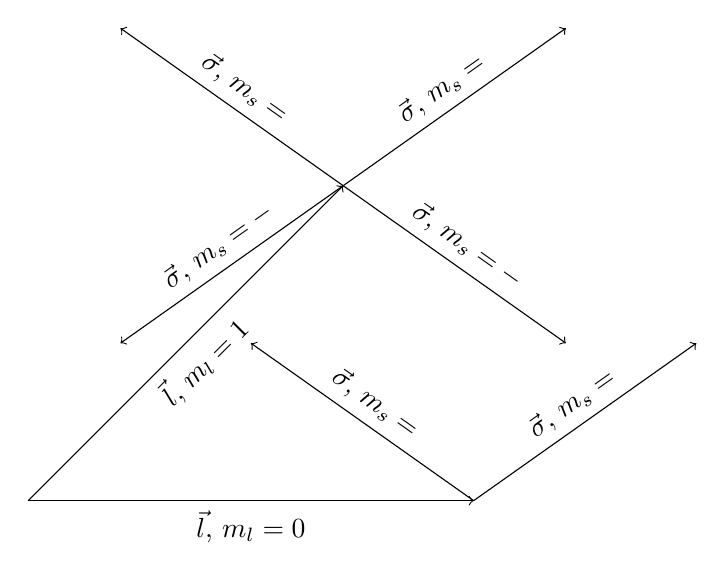
\begin{tikzpicture}[scale=4]
		\coordinate (l1) at (45:1.41421);
		\coordinate (l0) at (0:1.41421);
		\coordinate (l-1) at (-45:1.41421);

		\coordinate (s+l) at (144.736:0.866025);
		\coordinate (s+r) at (35.2644:0.866025);
		\coordinate (s-l) at (-144.736:0.866025);
		\coordinate (s-r) at (-35.2644:0.866025);

		\draw[->] (0, 0) -- (l1) node[midway, sloped, below] {$\vec l$, $m_l=1$};
		\draw[->] (0, 0) -- (l0) node[midway, sloped, below] {$\vec l$, $m_l=0$};

		\draw[->] (l0) -- ($(l0)+(s+r)$) node[midway, sloped, above] {$\vec \sigma$, $m_s=\half$};
		\draw[->] (l0) -- ($(l0)+(s+l)$) node[midway, sloped, above] {$\vec \sigma$, $m_s=\half$};
		\draw[->] (l1) -- ($(l1)+(s+r)$) node[midway, sloped, above] {$\vec \sigma$, $m_s=\half$};
		\draw[->] (l1) -- ($(l1)+(s+l)$) node[midway, sloped, above] {$\vec \sigma$, $m_s=\half$};

		\draw[->] (l1) -- ($(l1)+(s-r)$) node[midway, sloped, above] {$\vec \sigma$, $m_s=-\half$};
		\draw[->] (l1) -- ($(l1)+(s-l)$) node[midway, sloped, above] {$\vec \sigma$, $m_s=-\half$};
	\end{tikzpicture}
	\caption{%
		Alle Vektoren $\vec l$ und $\vec \sigma$ in einem Diagramm. Dabei habe
		ich die Fälle, in denen alle $z$-Komponenten umgekehrt sind,
		weggelassen, da sie letztlich das gleiche darstellen.
	}
	\label{fig:4/a/alle}
\end{figure}

\begin{figure}
	\centering
	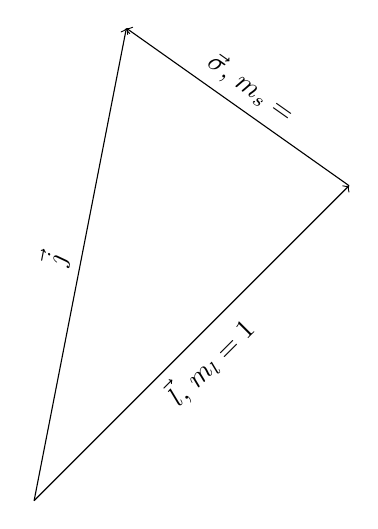
\begin{tikzpicture}[scale=4]
		\coordinate (l1) at (45:1.41421);
		\coordinate (l0) at (0:1.41421);
		\coordinate (l-1) at (-45:1.41421);

		\coordinate (s+l) at (144.736:0.866025);
		\coordinate (s+r) at (35.2644:0.866025);
		\coordinate (s-l) at (-144.736:0.866025);
		\coordinate (s-r) at (-35.2644:0.866025);

		\draw[->] (0, 0) -- (l1) node[midway, sloped, below] {$\vec l$, $m_l=1$};
		\draw[->] (l1) -- ($(l1)+(s+l)$) node[midway, sloped, above] {$\vec \sigma$, $m_s=\half$};
		\draw[->] (0, 0) -- ($(l1)+(s+l)$) node[midway, sloped, above] {$\vec j$};
	\end{tikzpicture}
	\caption{%
		$m_l = 1$ und $m_s = \half$
	}
	\label{fig:4/a/1}
\end{figure}

\begin{figure}
	\centering
	\begin{tikzpicture}[scale=4]
		\coordinate (l1) at (45:1.41421);
		\coordinate (l0) at (0:1.41421);
		\coordinate (l-1) at (-45:1.41421);

		\coordinate (s+l) at (144.736:0.866025);
		\coordinate (s+r) at (35.2644:0.866025);
		\coordinate (s-l) at (-144.736:0.866025);
		\coordinate (s-r) at (-35.2644:0.866025);

		\draw[->] (0, 0) -- (l1) node[midway, sloped, above] {$\vec l$, $m_l=1$};
		\draw[->] (l1) -- ($(l1)+(s+r)$) node[midway, sloped, above] {$\vec \sigma$, $m_s=\half$};
		\draw[->] (0, 0) -- ($(l1)+(s+r)$) node[midway, sloped, below] {$\vec j$};
	\end{tikzpicture}
	\caption{%
		$m_l = 1$ und $m_s = \half$
	}
	\label{fig:4/a/2}
\end{figure}

\begin{figure}
	\centering
	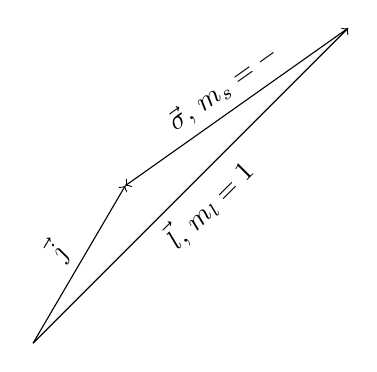
\begin{tikzpicture}[scale=4]
		\coordinate (l1) at (45:1.41421);
		\coordinate (l0) at (0:1.41421);
		\coordinate (l-1) at (-45:1.41421);

		\coordinate (s+l) at (144.736:0.866025);
		\coordinate (s+r) at (35.2644:0.866025);
		\coordinate (s-l) at (-144.736:0.866025);
		\coordinate (s-r) at (-35.2644:0.866025);

		\draw[->] (0, 0) -- (l1) node[midway, sloped, below] {$\vec l$, $m_l=1$};
		\draw[->] (l1) -- ($(l1)+(s-l)$) node[midway, sloped, above] {$\vec \sigma$, $m_s=-\half$};
		\draw[->] (0, 0) -- ($(l1)+(s-l)$) node[midway, sloped, above] {$\vec j$};
	\end{tikzpicture}
	\caption{%
		$m_l = 1$ und $m_s = -\half$
	}
	\label{fig:4/a/3}
\end{figure}

\begin{figure}
	\centering
	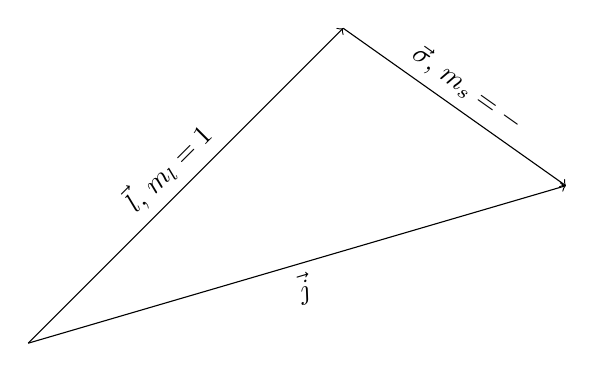
\begin{tikzpicture}[scale=4]
		\coordinate (l1) at (45:1.41421);
		\coordinate (l0) at (0:1.41421);
		\coordinate (l-1) at (-45:1.41421);

		\coordinate (s+l) at (144.736:0.866025);
		\coordinate (s+r) at (35.2644:0.866025);
		\coordinate (s-l) at (-144.736:0.866025);
		\coordinate (s-r) at (-35.2644:0.866025);

		\draw[->] (0, 0) -- (l1) node[midway, sloped, above] {$\vec l$, $m_l=1$};
		\draw[->] (l1) -- ($(l1)+(s-r)$) node[midway, sloped, above] {$\vec \sigma$, $m_s=-\half$};
		\draw[->] (0, 0) -- ($(l1)+(s-r)$) node[midway, sloped, below] {$\vec j$};
	\end{tikzpicture}
	\caption{%
		$m_l = 1$ und $m_s = -\half$
	}
	\label{fig:4/a/4}
\end{figure}

\begin{figure}
	\centering
	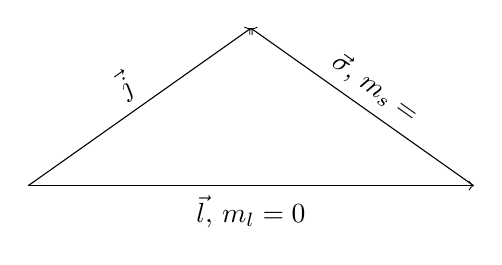
\begin{tikzpicture}[scale=4]
		\coordinate (l1) at (45:1.41421);
		\coordinate (l0) at (0:1.41421);
		\coordinate (l-1) at (-45:1.41421);

		\coordinate (s+l) at (144.736:0.866025);
		\coordinate (s+r) at (35.2644:0.866025);
		\coordinate (s-l) at (-144.736:0.866025);
		\coordinate (s-r) at (-35.2644:0.866025);

		\draw[->] (0, 0) -- (l0) node[midway, sloped, below] {$\vec l$, $m_l=0$};
		\draw[->] (l0) -- ($(l0)+(s+l)$) node[midway, sloped, above] {$\vec \sigma$, $m_s=\half$};
		\draw[->] (0, 0) -- ($(l0)+(s+l)$) node[midway, sloped, above] {$\vec j$};
	\end{tikzpicture}
	\caption{%
		$m_l = 0$ und $m_s = \half$
	}
	\label{fig:4/a/5}
\end{figure}

\begin{figure}
	\centering
	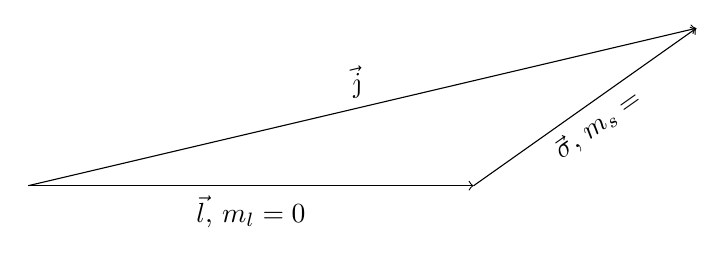
\begin{tikzpicture}[scale=4]
		\coordinate (l1) at (45:1.41421);
		\coordinate (l0) at (0:1.41421);
		\coordinate (l-1) at (-45:1.41421);

		\coordinate (s+l) at (144.736:0.866025);
		\coordinate (s+r) at (35.2644:0.866025);
		\coordinate (s-l) at (-144.736:0.866025);
		\coordinate (s-r) at (-35.2644:0.866025);

		\draw[->] (0, 0) -- (l0) node[midway, sloped, below] {$\vec l$, $m_l=0$};
		\draw[->] (l0) -- ($(l0)+(s+r)$) node[midway, sloped, below] {$\vec \sigma$, $m_s=\half$};
		\draw[->] (0, 0) -- ($(l0)+(s+r)$) node[midway, sloped, above] {$\vec j$};
	\end{tikzpicture}
	\caption{%
		$m_l = 0$ und $m_s = \half$
	}
	\label{fig:4/a/6}
\end{figure}

\subsection{Magnetische Momente}

Für die magnetischen Momente gilt:
\[
	\vec \mu_l = - \mu_B \vec l
	\eqnsep
	\vec \mu_s = - 2 \mu_B \vec \sigma
\]

Das magnetische Moment des Spins ist also im Vergleich zu den Drehmomenten
doppelt so groß wie das magnetische Moment des Spins. Daher ist die vektorielle
Summe $\vec \mu_j$ auch anders als $\vec j$.

In Abbildung \ref{fig:4/a/1} habe ich die magnetischen Momente eingetragen, das
Resultat ist in Abbildung \ref{fig:4/b/1}.

\begin{figure}
	\centering
	\begin{tikzpicture}[scale=4]
		\coordinate (l1) at (45:1.41421);
		\coordinate (l0) at (0:1.41421);
		\coordinate (l-1) at (-45:1.41421);

		\coordinate (mul1) at (l1);

		\coordinate (s+l) at (144.736:0.866025);
		\coordinate (s+r) at (35.2644:0.866025);
		\coordinate (s-l) at (-144.736:0.866025);
		\coordinate (s-r) at (-35.2644:0.866025);

		\coordinate (mus+l) at (144.736:1.73205);

		\draw[->, dotted] (0, 0) -- (l1) node[midway, sloped, below] {};
		\draw[->, dotted] (l1) -- ($(l1)+(s+l)$) node[midway, sloped, above] {};
		\draw[->] (0, 0) -- ($(l1)+(s+l)$) node[midway, sloped, above] {$\vec j$};

		\draw[->] (0, 0) -- (mul1) node[midway, sloped, below] {$\vec \mu_l$};
		\draw[->] (mul1) -- ($(mul1)+(mus+l)$) node[midway, sloped, above] {$\vec \mu_s$};
		\draw[->] (0, 0) -- ($(mul1)+(mus+l)$) node[midway, sloped, above] {$\vec \mu_j$};
	\end{tikzpicture}
	\caption{%
		$m_l = 1$ und $m_s = \half$
	}
	\label{fig:4/b/1}
\end{figure}

In dieser Abbildung ist dann auch zu sehen, dass $\vec j \nparallel \vec\mu_j$
gilt.

%%%%%%%%%%%%%%%%%%%%%%%%%%%%%%%%%%%%%%%%%%%%%%%%%%%%%%%%%%%%%%%%%%%%%%%%%%%%%%%
%                                    Ende                                     %
%%%%%%%%%%%%%%%%%%%%%%%%%%%%%%%%%%%%%%%%%%%%%%%%%%%%%%%%%%%%%%%%%%%%%%%%%%%%%%%

\IfFileExists{\bibliographyfile}{
	%\bibliography{\bibliographyfile}
}{}

\end{document}

% vim: spell spelllang=de
